\subsection{Root and Copy Protection} \label{subsection:android-copyroot}
"Rooting" or "getting root" is the process of modifying the operation system's software that shipped with a device in order to get complete control over it.
The name "root" comes from the Linux \gls{os} world where the user \textit{root} has all privileges.
This allows to overcome limitations set by carriers and manufacturers, like removing pre-installed applications, extending system functionality or to upgrading to custom versions of Android.
Manufacturers and carriers do not approve of rooting but they cannot prevent it as the access is usually gained by exploiting vulnerabilities in the system's code or device drivers.
Vulnerabilities are quite common.
As seen in figure~\ref{fig:root}, there have been over 30 vulnerabilities to gain root rights since Febraury 2015.
Details and references of these can be accessed on pages like Common Vulnerabilities and Exposures or similar \cite{cveAndroidPriv} \cite{cveDetails}.
\newline
\begin{figure}[h]
    \centering
    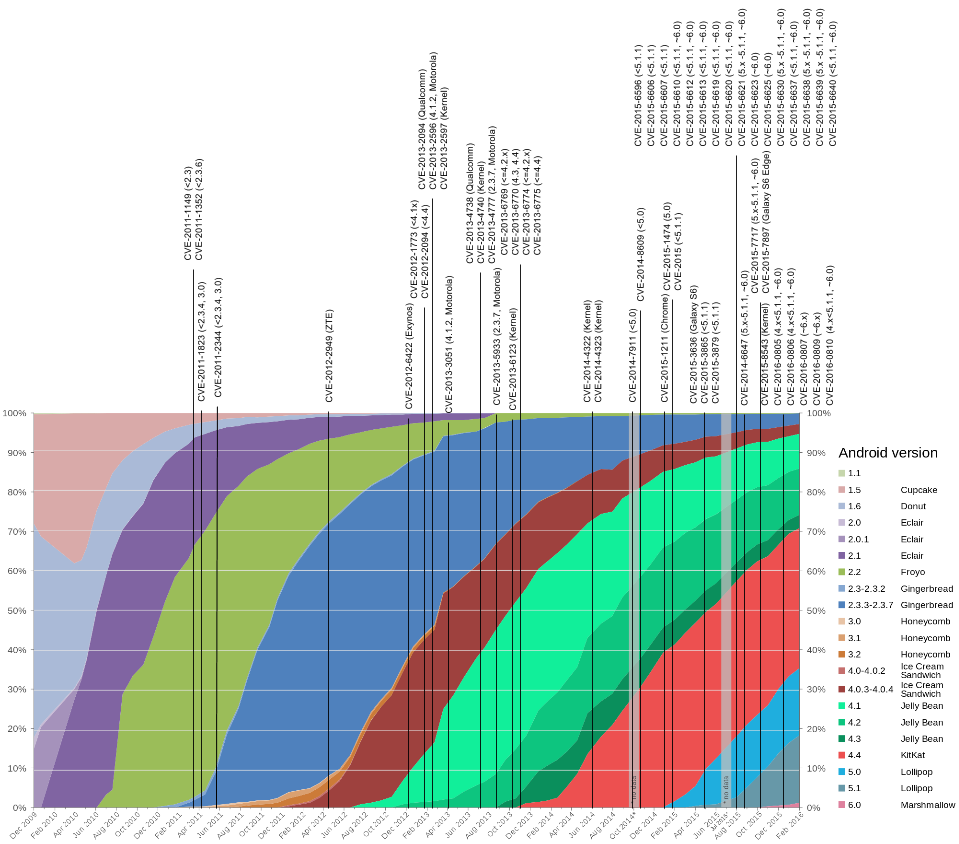
\includegraphics[width=1\textwidth]{data/timeline.png}
    \caption{Timeline of market share of evolving Android versions and dates of root exploits recorded \cite{distributionRoot} \cite{androidVulnerabilities} \cite{cveAndroidPriv} \cite{cveDetails}}
    \label{fig:root}
\end{figure}
Today it is easy to exploit these vulnerabilities and gain root rights, even for non-techies.
There are videos and tutorials available on the internet, even tools to automate the process, like Wugfresh's Rootkits \cite{wugfresh}.
Rooting is usually bundled with installing a program called \textit{su} which manages the root access for applications requesting it.
Rooting a phone is not without risk since installing bad files can result in the so called \textit{bricking} meaning the phone is nonfunctional since the software cannot be executed anymore. \cite{androidpoliceRoot}
\newline
Now that the application is installed and ready to run.
Copy protection is applied to prevent unauthorized usage of the app.
The downloaded \gls{apk}, purchased from an application store, is moved to \textit{/mnt/app-asec/package.name} on the phone.
The user has no rights to access the cotaining \gls{apk} and thus cannot copy it.
This mechanism has a major flaw, as copy protection is circumvented when a single user can get hold of the application and redistribute it, e.g. by using root.
This was effective in the early days of Android when rooting was not easily facilitated.
\newline
Since rooting circumvents the copy protection, it is declared as deprecated and new ways of protecting applications have to been invented.
